\documentclass[12pt]{article}
\usepackage{graphicx}
\usepackage{hyperref}
\pagestyle{empty}
\setcounter{secnumdepth}{2}

\topmargin=0cm
\oddsidemargin=0cm
\textheight=22.0cm
\textwidth=16cm
\parindent=0cm
\parskip=0.15cm
\topskip=0truecm
\raggedbottom
\abovedisplayskip=3mm
\belowdisplayskip=3mm
\abovedisplayshortskip=0mm
\belowdisplayshortskip=2mm
\normalbaselineskip=12pt
\normalbaselines

\begin{document}

\vspace*{0.5in}
\centerline{\bf\Large FunSheets Software}

\vspace*{0.5in}
\centerline{\bf\Large Team 2 - Iteration 2}

\vspace*{0.5in}
\centerline{\bf\Large 4 March 2013}

\vspace*{1.5in}
\begin{table}[htbp]
\caption{Team}
\begin{center}
\begin{tabular}{|r | c|}
\hline
Name & ID Number \\\hline\hline
Kevin Cameron & 9801448 \\\hline\hline
Addison Rodomista & 1967568 \\\hline\hline
Dragos Dinulescu & 6304826 \\\hline\hline
Adrian Max McCrea & 9801448 \\\hline\hline
Ghazal Zamani & 1971158 \\\hline\hline
Karim Kaidbey & 9654726 \\\hline\hline
Carmelo Fragapane & 6298265 \\\hline\hline
Long Wang & 9547967 \\\hline\hline
Simone Ovilma & 9112510 \\\hline\hline
Nicholas Constantinidis & 6330746 \\\hline\hline
Asmaa Alshaibi & 9738231 \\\hline
\end{tabular}
\end{center}
\end{table}

\clearpage

\section{Introduction}
This document is the project design document. As the name suggest this document will basically refer to the design that went behind the creating of this program. The goal of this document is to familiarise the reader with the thought process and planning that went into deciding how the program should be made. The document will introduce the overall architectural design of the FunSheets program as well as a more detailed look into the design of the subsystems, followed by some dynamic design scenario of the program.

\section{Architectural Design}
This section gives a high-level description of the deliverable 2 system in terms of its modules and their respective purpose and exact interfaces. You will also find the updated and detailed version of the architecture design that was presented in deliverable 1 for our FunSheet spreadsheet application.
\subsection{Architecture Diagram}
\begin{figure}[htbp]
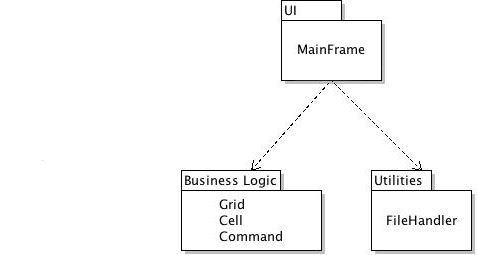
\includegraphics[scale=.7]{packagediagram.jpg}
\caption{High-Level Structure Package Diagram}
\label{fig:High-Level-Structure-Package-Diagram}
\end{figure}
The rationale behind this design was to create a separation between the model and the view. By separating the model and view we are decoupling these objects so that changes to one can affect any number of others without requiring the changed object to know details of the others.\\\\
This iteration's design is drastically different from that in deliverable 1. In the deliverable 1 design the team focused solely on a functioning simple application that got the job done. In this deliverable we designed it with functionality, reusability, and cleanliness in mind.\\\\
In this deliverable the system consists of three separate subsystems. These subsystems are the UI or view, the business logic or model, and then finally the utilities. The UI represents what the user sees and how they interact with the system. The model is the behind the scenes operations of the system. This means handling the inputted formulas passed by the view, performing some validation on the formula, formulating the proper result, and then giving the result to the view to be displayed. The utilities includes the necessary miscellaneous functions required by the system. In this case the only current function is the loading and saving of the spreadsheets.

\subsection{Subsystem Interfaces Specifications}
The following subsections describe the interfaces between the subsystems. This includes the function call, the service of the function, the parameters that are passed in order to have a service fullfilled, and finally the valid ranged of values accepted by the functions.
\subsubsection{UI Subsystem Interface}
The UI Subsystem never gets called open for any services, it does however use the other subsystem interfaces.
\subsubsection{Business Logic Subsystem Interface}

\begin{tabular}{|p{4.75cm}|p{11.25cm}|}
\hline
\textbf{Function Call} & Grid()
\\\hline
\textbf{Service} & Initializes the grid object.
\\\hline
\end{tabular}

\begin{tabular}{|p{4.75cm}|p{11.25cm}|}
\hline
\textbf{Function Call} & getSelectedRow()
\\\hline
\textbf{Service} & Returns the spreadsheet's currently selected row.
\\\hline
\textbf{Return Description} & The spreadsheet's currently selected row.
\\\hline
\end{tabular}

\begin{tabular}{|p{4.75cm}|p{11.25cm}|}
\hline
\textbf{Function Call} & getSelectedColumn()
\\\hline
\textbf{Service} & Returns the spreadsheet's currently selected column.
\\\hline
\textbf{Return Description} & The spreadsheet's currently selected column.
\\\hline
\end{tabular}

\begin{tabular}{|p{4.75cm}|p{11.25cm}|}
\hline
\textbf{Function Call} & insertValue(double value, int row, int column)
\\\hline
\textbf{Service} & Inserts the given value into the given row and column.
\\\hline
\textbf{Parameter Description} & The value to be inserted and the integer row and column that will be inserted into.
\\\hline
\textbf{Parameter Constraints} & Both the row and column should be between 0 and 10 inclusive.
\\\hline
\end{tabular}

\begin{tabular}{|p{4.75cm}|p{11.25cm}|}
\hline
\textbf{Function Call} & insertValue(String value, int row, int column)
\\\hline
\textbf{Service} & Inserts the given value into the given row and column.
\\\hline
\textbf{Parameter Description} & The string value to be inserted, and the integer row and column that will be inserted into.
\\\hline
\textbf{Parameter Constraints} & Both the row and column should be between 0 and 10 inclusive.
\\\hline
\end{tabular}

\begin{tabular}{|p{4.75cm}|p{11.25cm}|}
\hline
\textbf{Function Call} & evaluateCell(Cell cell)
\\\hline
\textbf{Service} & Takes the given cell and analyzes its contents to see if it is a primitive or a string. If it is a primitive it simply sets the cell's value to the primitive. If it is a string it evaluates the formula and sets the cell's value to the corresponding result.
\\\hline
\textbf{Parameter Description} & The cell whose contents will be evaluated.
\\\hline
\textbf{Return Description} & The double result of the evaluation.
\\\hline
\end{tabular}

\begin{tabular}{|p{4.75cm}|p{11.25cm}|}
\hline
\textbf{Function Call} & getRowCount()
\\\hline
\textbf{Service} & Gets the current number of rows.
\\\hline
\textbf{Return Description} & The current number of rows.
\\\hline
\end{tabular}

\subsubsection{Utilities Subsystem Interface}

\begin{tabular}{|p{4.75cm}|p{11.25cm}|}
\hline
\textbf{Function Call} & FileHandler(Component component)
\\\hline
\textbf{Service} & Initializes the FileHandler object.
\\\hline
\textbf{Parameter Description} & The component that the FileHandler will operate on.
\\\hline
\end{tabular}

\begin{tabular}{|p{4.75cm}|p{11.25cm}|}
\hline
\textbf{Function Call} & saveFile(Grid grid)
\\\hline
\textbf{Service} & Saves the given spreadsheet to the user's chosen destination. 
\\\hline
\textbf{Parameter Description} & The grid in which represents the spreadsheet and its contents.
\\\hline
\end{tabular}

\begin{tabular}{|p{4.75cm}|p{11.25cm}|}
\hline
\textbf{Function Call} & loadFile(Grid grid)
\\\hline
\textbf{Service} & Loads the given spreadsheet to the user's chosen destination. 
\\\hline
\textbf{Parameter Description} & The grid in which represents the spreadsheet and its contents.
\\\hline
\end{tabular}

\begin{tabular}{|p{4.75cm}|p{11.25cm}|}
\hline
\textbf{Function Call} & setSaved(Boolean saved)
\\\hline
\textbf{Service} & Signifies whether the current open spreadsheet is saved or not.
\\\hline
\textbf{Parameter Description} & True if the currently open spreadsheet is saved, false otherwise.
\\\hline
\end{tabular}

\begin{tabular}{|p{4.75cm}|p{11.25cm}|}
\hline
\textbf{Function Call} & checkSaved()
\\\hline
\textbf{Service} & Returns a boolean representing whether the current open spreadsheet is saved or not.
\\\hline
\textbf{Return Description} & True if the currently open spreadsheet is saved, false otherwise.
\\\hline
\end{tabular}

\section{Detailed Design}

\subsection{Subsystem \textless Spreadsheet Logic\textgreater}
\subsubsection{Detailed Design Diagram}
The rational behind this design was to make the subsystem this way was to simplify writing the code as well as improving it's overall comprehensiveness as many people would be using it an need to understand it. To achieve this it was split into three classes Cell, Grid and Command. Cell is the base unit that makes up Grid. Command is used to read formulas and apply them from a Cell.
\begin{figure}[ht!]
\centering
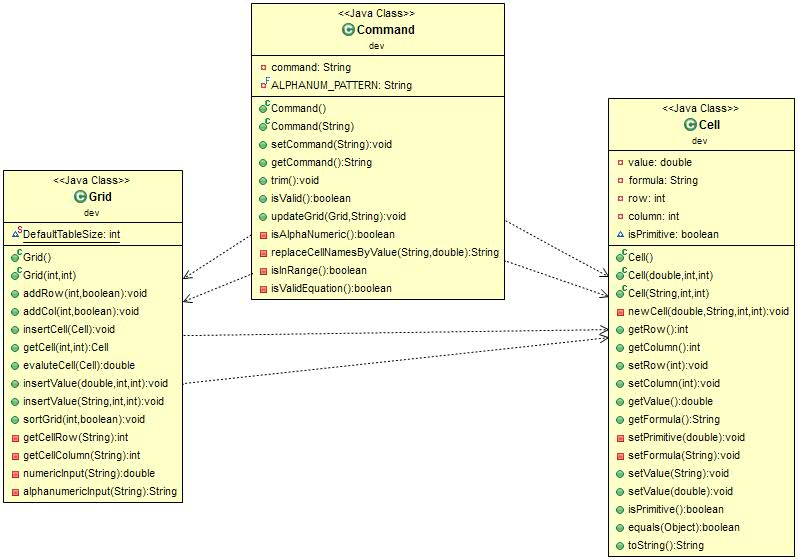
\includegraphics[width=165mm]{SS1_Spreadsheet.jpg}
\end{figure}

\subsubsection{Units Description}
Cell class is a class that stores: a value(value), a formula(formula), a row(row), a column(column), and a primitive identifier(isPrimitive). Most of the items just listed are self-explaining but elaboration may be needed on isPrimitive; it is basically an identifier to indicate weather the cell is simply holding a value (true) or it is following a formula (false).

The Grid class is fairly simple it simply creates a two-dimensional array of Cell that is sized at DefaultTableSize by DefaultTableSize.

Command class is used to take formulas from non-primitive Cells and apply them to obtain a value.


\subsection{Subsystem \textless Graphic User Interface\textgreater}
\subsubsection{Detailed Design Diagram}
The rational behind designing the subsystem this way was to keep the whole graphic user interface in one class so it could be easily understood and manipulated by everyone working on it in the future.
\begin{figure}[ht!]
\centering
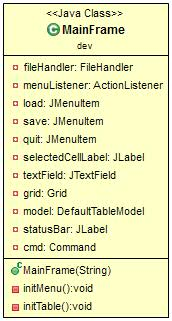
\includegraphics[width=45mm]{SS2_GUI.jpg}
\end{figure}

\subsubsection{Units Description}
Basically this creates a window with a menu bar that contains commands to save load and quit. Under the menu it has an input line for the a 10 by 10 grid below it. At the bottom of the window there is a status bar that is used to communicate with a user. 

\subsection{Subsystem \textless Save \& Load\textgreater}
\subsubsection{Detailed Design Diagram}
This Subsystem was designed by keeping the function simple to program for the developer. This is achieve though the use of already existing classes from Java swing, most notably JFileChooser.
\begin{figure}[ht!]
\centering
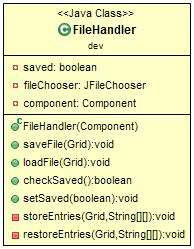
\includegraphics[width=40mm]{SS3_SaveLoad.jpg}
\end{figure}

\subsubsection{Units Description}
This subsection allows for a user to browse through their file system to select a location to save the currently opened grid or load an existing grid. Files are saved in .cvs format, the advantage of this is that it is a recognized format and can be opened with other programs such as excel or even a standard text editor but the disadvantage is that the currently working grid will not save the formula of cells but rather only their values. 

\section{Dynamic Design Scenarios}
[Describe some (at least two) important execution scenarios of the system using UML sequence diagrams. These scenarios must demonstrate how the various subsystems and units are interacting to achieve a system-level service. Units and subsystems depicted here must be compatible with the descriptions provided in section 2 and 3.]  

\end{document}
